\section{Nested hierarchy as the random variability structure}
\label{sec:variabilityModel}
\label{math:variability}

This section describes the variability structure of the random effects and the related naming convention. It is largely based on the discussions and conclusions from the Copenhagen focus meeting \cite{Copenhagen:2013}. Accordingly, in the following we will distinguish: 
\begin{itemize}
\item
(related to the observations) -- \textit{residual variability}, also known as \textit{intra-individual variability} and
\item
(related to the parameters) -- \textit{inter-individual} and \textit{inter-occasion variabilities}
\end{itemize}
The former is described in the section \ref{sec:residualErrorModel}, while the latter is described in this section.

\begin{figure}[htb!]
\centering
  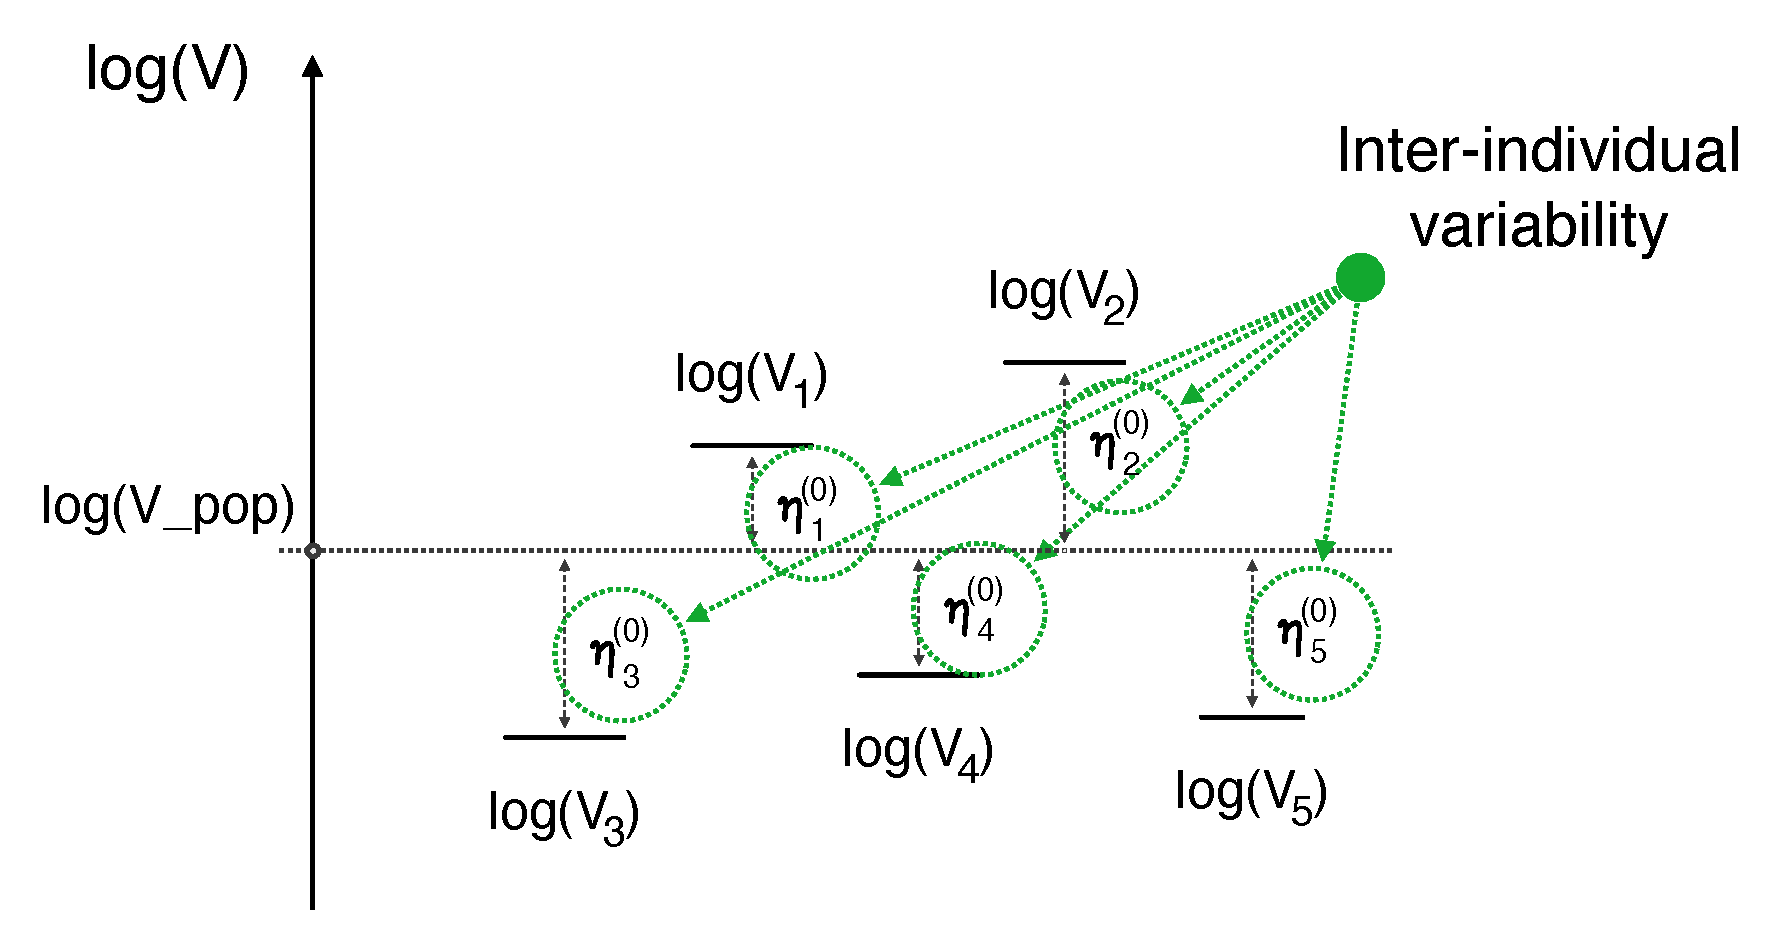
\includegraphics[width=95mm]{pics/Subject-level.pdf}
 \caption{Inter-individual variability typically occurring in an experiment, here $\log(V_{i=1\cdots5})$ i.e. values for five subjects, varying around a typical value $\log(V_{pop})$, are shown.}
 \label{fig:subjectLevelVariability}
\end{figure}

\begin{figure}[htb!]
\centering
  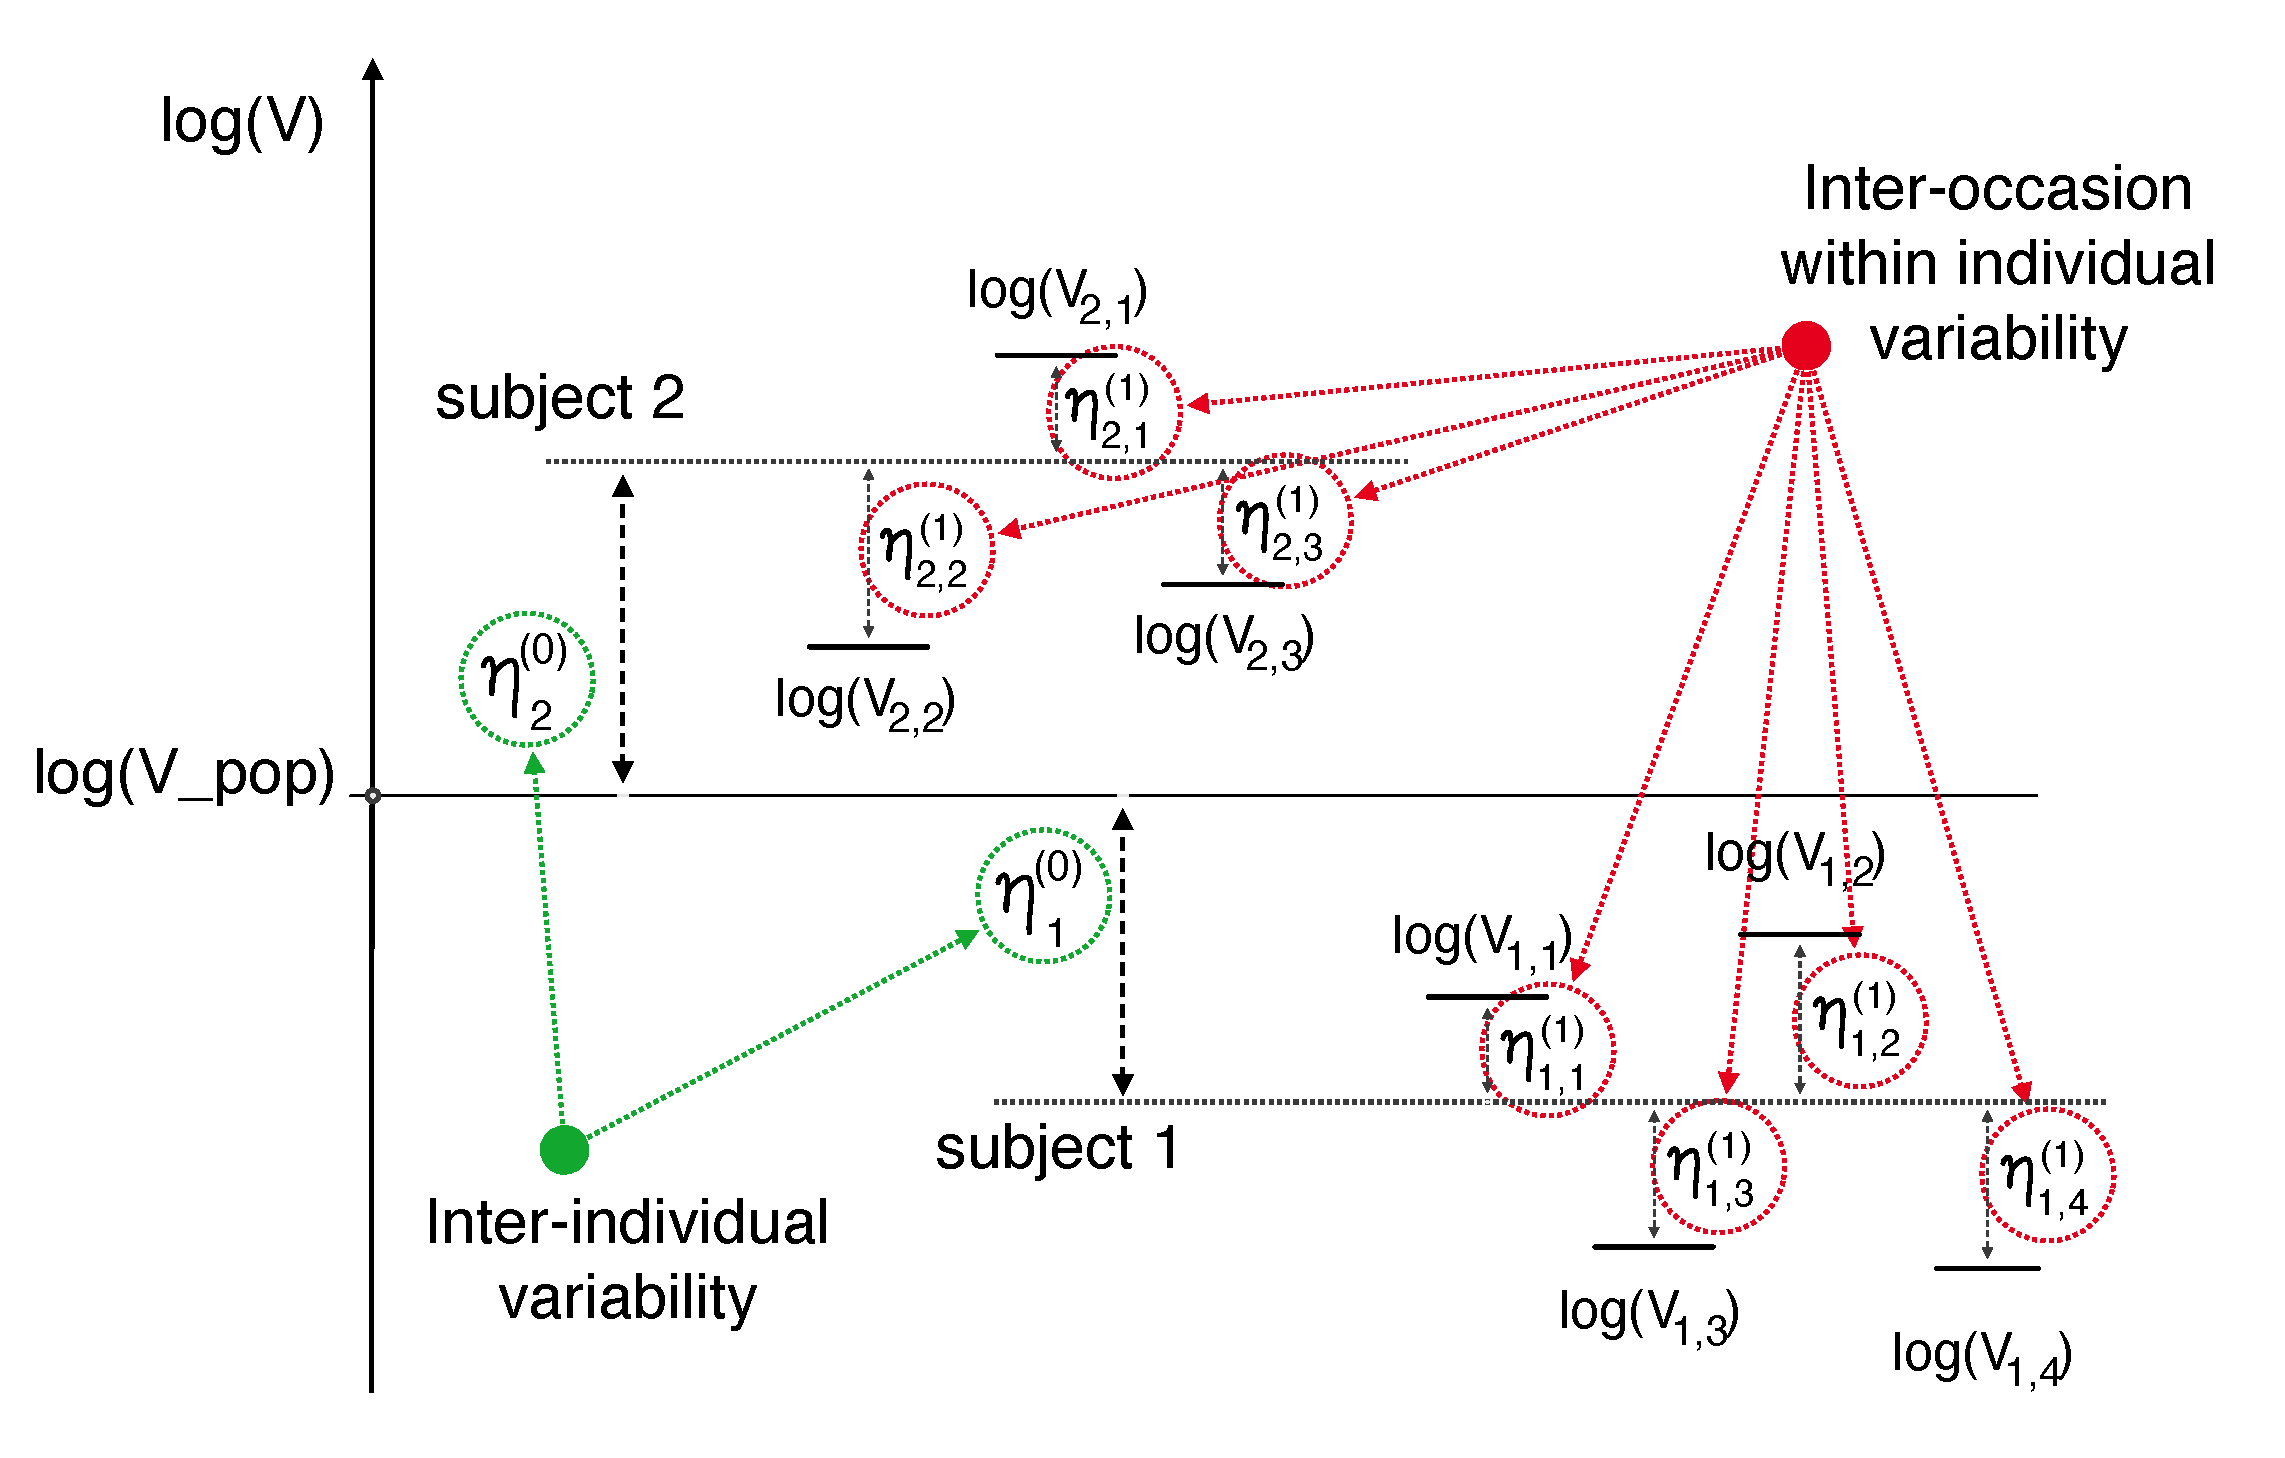
\includegraphics[width=120mm]{pics/Subject-occasion-level.pdf}
 \caption{Subject variability level, $(0)$, and within-subject (or occasion) variability level, $(1)$, typically occurring in an experiment, with index $i$ for subjects and $k$ for occasion. Here two subjects only are visualised, each of them having four or three occasions, respectively.}
 \label{fig:subjectOccasionLevelVariability}
\end{figure}

\subsection{Motivation}
One way to look at variability is to consider the following simple experiment: in this 
experiment, we estimate the volume of distribution in five subjects. Following a drug 
administration we collect blood samples over a time interval and estimate each 
subject's PK parameters. The result will be a set of five individual estimates such 
as those in Figure \ref{fig:subjectLevelVariability}. The values vary around a certain 
typical/population value. It is apparent that the only variability source is the fact that 
these are different persons, i.e. we have a rough estimate of the so called 
\textit{inter-individual} variability.\\
As an extension of this setup, we can now consider different number of occasions, 
when the PK parameters are estimated for each subject. If we restrict the discussion 
to two subjects only, each of them having three or four occasions, respectively, we 
can illustrate the results such those in Figure \ref{fig:subjectOccasionLevelVariability}. 
Repeatedly performing the same experiment for each subject is equivalent to create 
an additional level of variability, the \textit{inter-occasion within individual} variability.\\ 
Similarly, one can add e.g. 'country' or 'study centre' as new variability levels. 
If a clinical trial has been conducted in various countries or centres, it is reasonable 
to ask if the geographic location influences the outcome of the study. 

\subsection{General case}
As a generalisation of the examples described above, one can derive the 
\textit{nested hierarchy} (also known as \textit{inclusion hierarchy}) of the variability 
structure of random effects. It can be visualised as a tree or alternatively using 
a Venn diagram, see Figures \ref{IOVgeneral_tree} and \ref{IOVgeneral_venn}. \\
The tree representation consists of \textit{nodes} and \textit{links} or \textit{edges}. 
It has the advantage that it visualises the whole structure explicitly from the top 
level, the \textit{root} node, down to lowest level of the variability. It provides 
immediate insights needed to understand or to verify the setup of a trial design. 
However, in case of a very complex structure, with high number of levels and/or 
subjects, it can become very large, making the tree difficult to represent in a typical 
document. It this case showing only partial branches will be more helpful, 
e.g. Figure \ref{IOVgeneral_tree}. On the contrary, the Venn diagram visualises 
the levels only, and it might be more suited for the complex cases. Usually, the 
variability structure consists of only one or two levels, e.g. \textit{individual} or 
\{\textit{individual}, \textit{occasion}\}, see examples below. 


The \textit{root}, i.e. the top node in the tree structure, stands for the population/typical 
value of a parameter. Following the current nomenclature, every subsequent variability 
level is either 'positive' or 'negative' dependent on its position relative to the reference 
'subject level', denoted as 0 -- the level 'zero'. Each level has a covariance matrix 
associated with it, i.e. 
\begin{itemize}
\item 
$\Omega^{-n}$ -- for levels above the reference level -- their names will vary according to 
the nature of the levels. For example the variability on country level is called 
'between-country variability'.
\item 
$\Omega^0$ -- reference level\footnote{Target tools such as NONMEM or Monolix assume 
the subject level as the reference level by default. \pml doesn't make such assumption and 
the \emph{zero} level can be explicitly defined and is required if more then one level exist.}, 
also called BSV (between subject variability) or IIV (inter-individual variability).
\item 
$\Omega^{+n}$ -- for levels below the reference level -- called  IOV (inter-occasion variability) or
WSV (within-subject variability).
\end{itemize}
The number of levels will vary dependent on the nature of the study. Cases without or 
with only positive/negative levels are possible. Please note that \pharmml doesn't require 
numbers to be assigned to the various levels of variability. Instead the user can 
define meaningful identifiers.

\begin{figure}[htb!]
\centering
  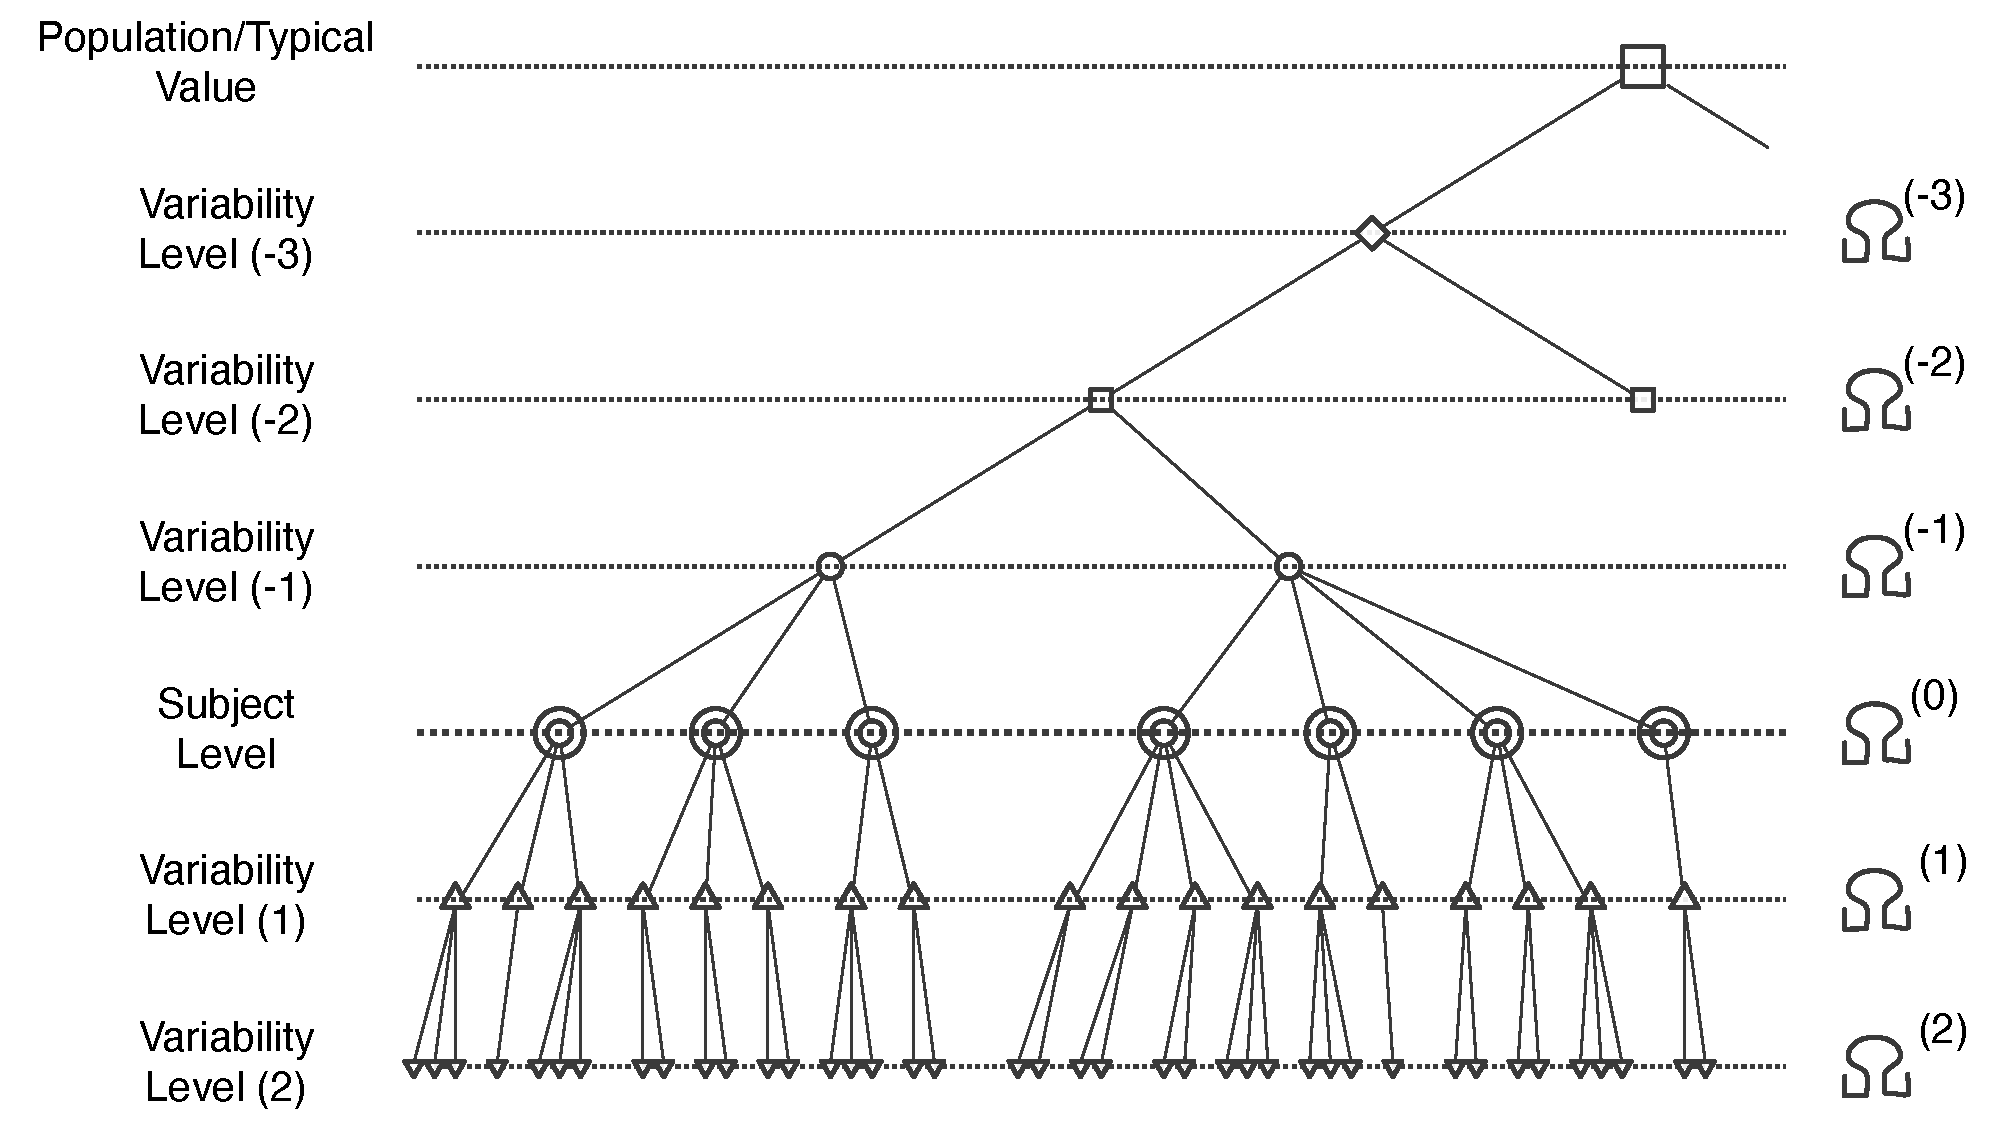
\includegraphics[width=130mm]{pics/IOV-general-TREE}
 \caption{General nested hierarchy of the variability structure -- as tree. Note that 
 \pharmml doesn't require or use numbers to be assigned to the various levels of 
 variability. Instead the user can define meaningful identifiers such as \emph{subject}
  or \emph{iiv} for level (0), \emph{occasion} or \emph{iov} for level (1), \emph{study} for level (-1) etc.}
 \label{IOVgeneral_tree}
\end{figure}

\begin{figure}[htb!]
\centering
  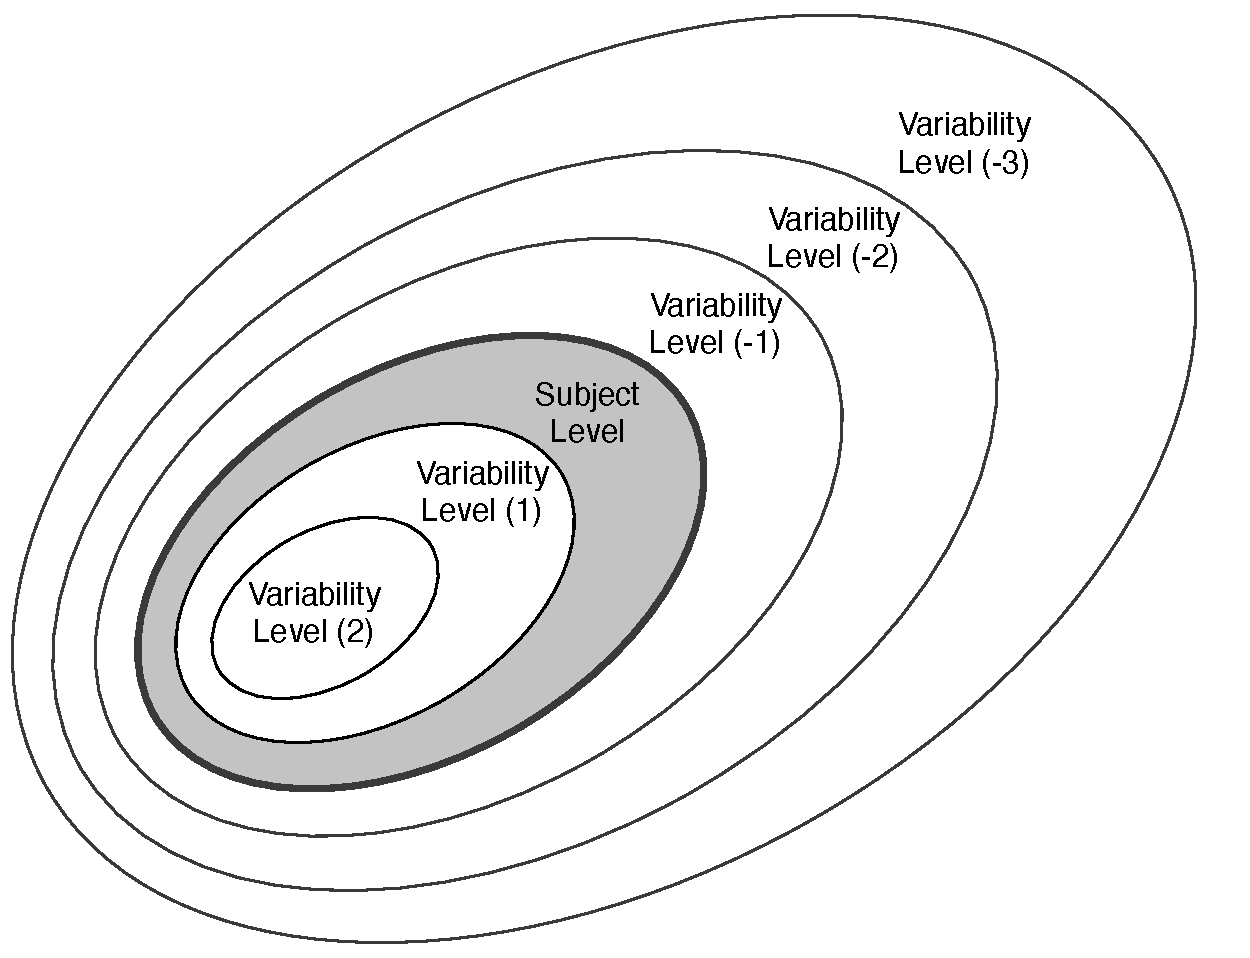
\includegraphics[width=90mm]{pics/IOV-general-VENN}
 \caption{General nested hierarchy of the variability structure -- as Venn diagram.}
 \label{IOVgeneral_venn}
\end{figure}


\paragraph{Example 1}
This example handles the simplest scenario, with only one level of variability: \textit{subject}--level, see Figure \ref{tree_IOV0}. The following symbols are used
\begin{itemize}
\item
$i$ -- subject index, $1\le i \le N$
\end{itemize} 
with $N_l$ -- number of subjects.\\
The typical parameter model, without covariate, reads as follows:
\begin{align*}
& \log(V_i) = \log(V_{pop}) + \eta_i^{(0)}  
\end{align*} 
or alternatively:
\begin{align*}
& V_i = V_{pop} \,e^{\eta_i^{(0)}}  
\end{align*} 
with $\eta_i^{(0)} \sim \mathcal{N}\big(0,\Omega^{(0)}\big)$.


\begin{figure}[htb!]
\centering
  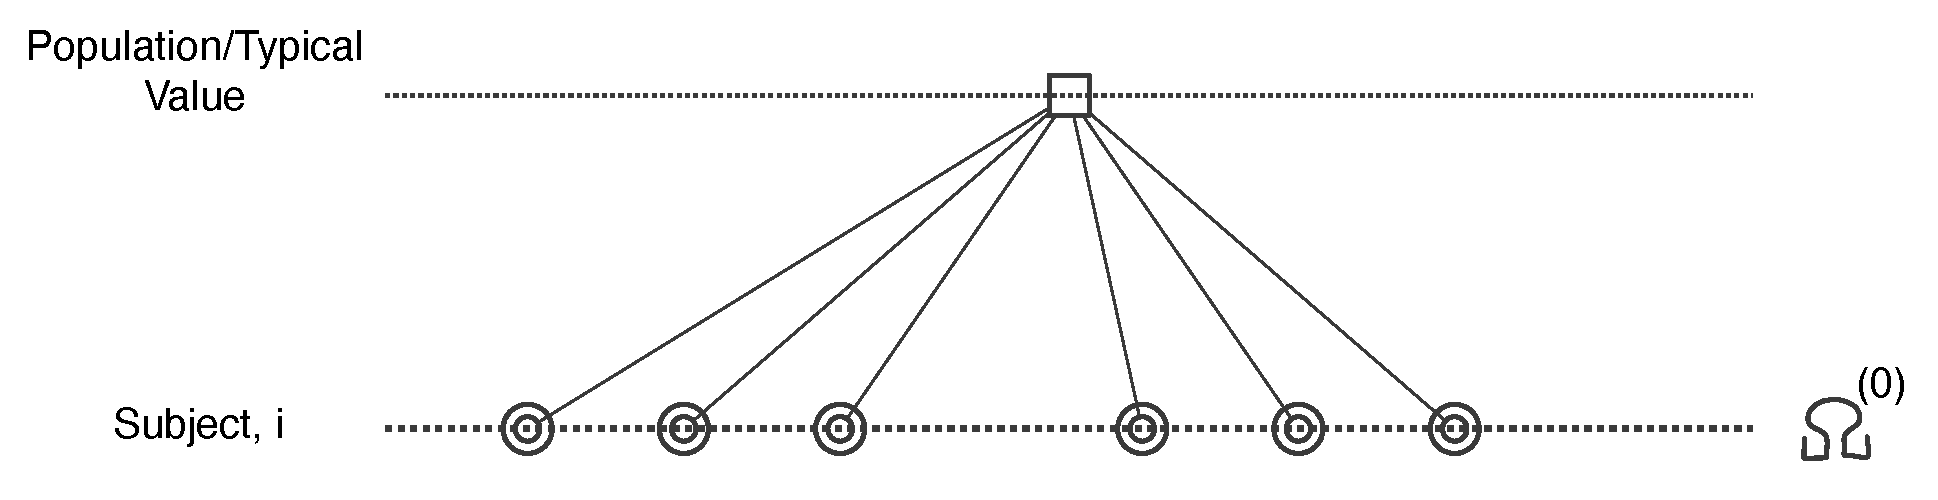
\includegraphics[width=120mm]{pics/tree_IOV0}
 \caption{Example 1 -- single level of variability: \textit{subject} -- (0) level.}
 \label{tree_IOV0}
\end{figure}

\paragraph{Example 2}
In this example there are three levels of variability: \{\textit{centre, subject, occasion}\}, see Figure \ref{tree_IOV1}. Following symbols are used:
\begin{itemize}
\item
$l$ -- centre index, $1\le l \le L$
\item
$i$ -- subject index, $1\le i \le N_l$
\item
$k$ -- occasion index, $1\le k \le N_{li}$
\end{itemize} 
with
\begin{itemize}
\item
$L$ -- number of centres
\item
$N_l$ -- number of subjects in centre \textit{l}
\item
$N_{li}$ -- number of occasions in subject \textit{i} in centre \textit{l}
\end{itemize} 
The parameter model, without covariate, reads as follows:
\begin{align*}
& \log(V_{lik}) = \log(V_{pop}) + \eta_l^{(-1)} + \eta_{li}^{(0)} + \eta_{lik}^{(+1)}  
\end{align*} 
or alternatively:
\begin{align*}
& V_{lik} = V_{pop} \, e^{\eta_l^{(-1)}} e^{\eta_{li}^{(0)}} e^{\eta_{lik}^{(+1)}}  
\end{align*} 
with
\begin{align*}
 & \eta_l^{(-1)} \sim \mathcal{N}\big(0,\Omega^{(-1)}\big), \quad \eta_{li}^{(0)} \sim \mathcal{N}\big(0,\Omega^{(0)}\big),
\quad \eta_{lik}^{(+1)} \sim \mathcal{N}\big(0,\Omega^{(+1)}\big) 
\end{align*}


\begin{figure}[htb!]
\centering
  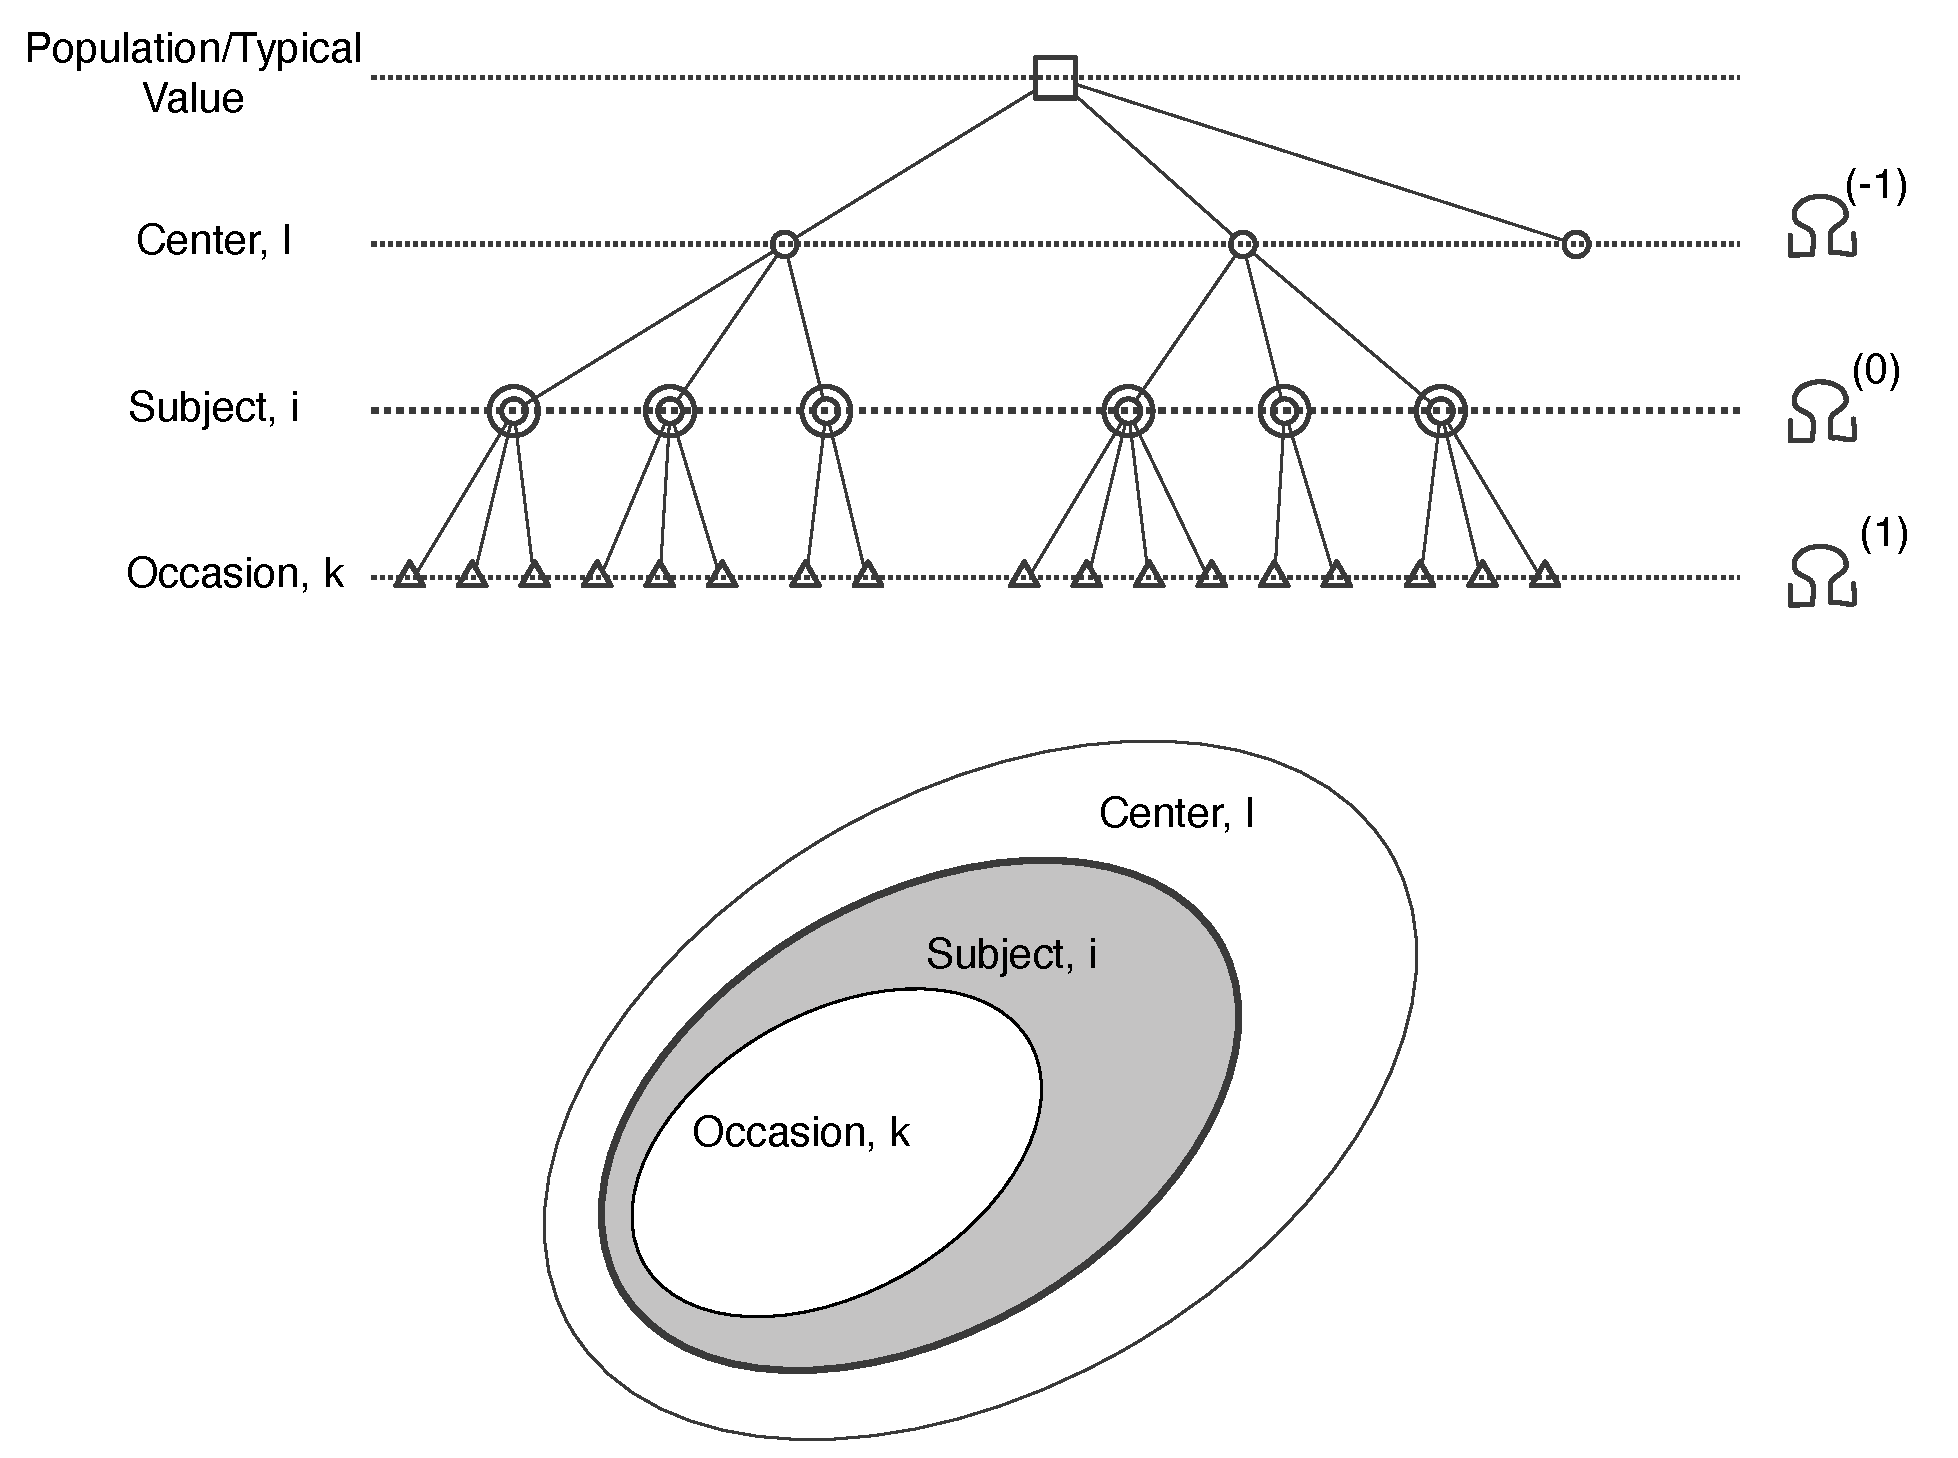
\includegraphics[width=120mm]{pics/tree_IOV1}
 \caption{Example 1 -- three levels of variability: \{\textit{centre (+1), subject (0), occasion (-1)}\}}
 \label{tree_IOV1}
\end{figure}


\paragraph{Example 3}
In this example there are four levels of variability: \{\textit{country, centre, subject, occasion}\}, see Figure \ref{tree_IOV2}. The symbol list is extended by one for 'country' as follows:
\begin{itemize}
\item
$m$ -- country index, $1\le m \le M$
\item
$l$ -- centre index, $1\le l \le N_m$
\item
$i$ -- subject index, $1\le i \le N_{ml}$
\item
$k$ -- occasion index, $1\le k \le N_{mli}$
\end{itemize} 
with
\begin{itemize}
\item
$M$ -- number of countries
\item
$N_m$ -- number of centres in country \textit{m}
\item
$N_{ml}$ -- number of subjects in centre \textit{l} in country \textit{m}
\item
$N_{mli}$ -- number of occasions in subject \textit{i} in centre \textit{l} in country \textit{m}
\end{itemize} 
The parameter model reads as follows:
\begin{align*}
& \log(V_{mlik}) = \log(V_{pop}) + \eta_m^{(-2)} + \eta_{ml}^{(-1)} + \eta_{mli}^{(0)} + \eta_{mlik}^{(+1)}  
\end{align*} 
or alternatively:
\begin{align*}
& V_{mlik} = V_{pop} \, e^{\eta_m^{(-2)}} e^{\eta_{ml}^{(-1)}} \; e^{\eta_{mli}^{(0)}} \; e^{\eta_{mlik}^{(+1)}}  
\end{align*} 
with
\begin{align*}
 & \eta_m^{(-2)} \sim \mathcal{N}\big(0,\Omega^{(-2)}\big), \quad \eta_{ml}^{(-1)} \sim \mathcal{N}\big(0,\Omega^{(-1)}\big), \quad
 \eta_{mli}^{(0)} \sim \mathcal{N}\big(0,\Omega^{(0)}\big), \quad \eta_{mlik}^{(+1)} \sim \mathcal{N}\big(0,\Omega^{(+1)}\big) 
\end{align*} 



\begin{figure}[htb!]
\centering
  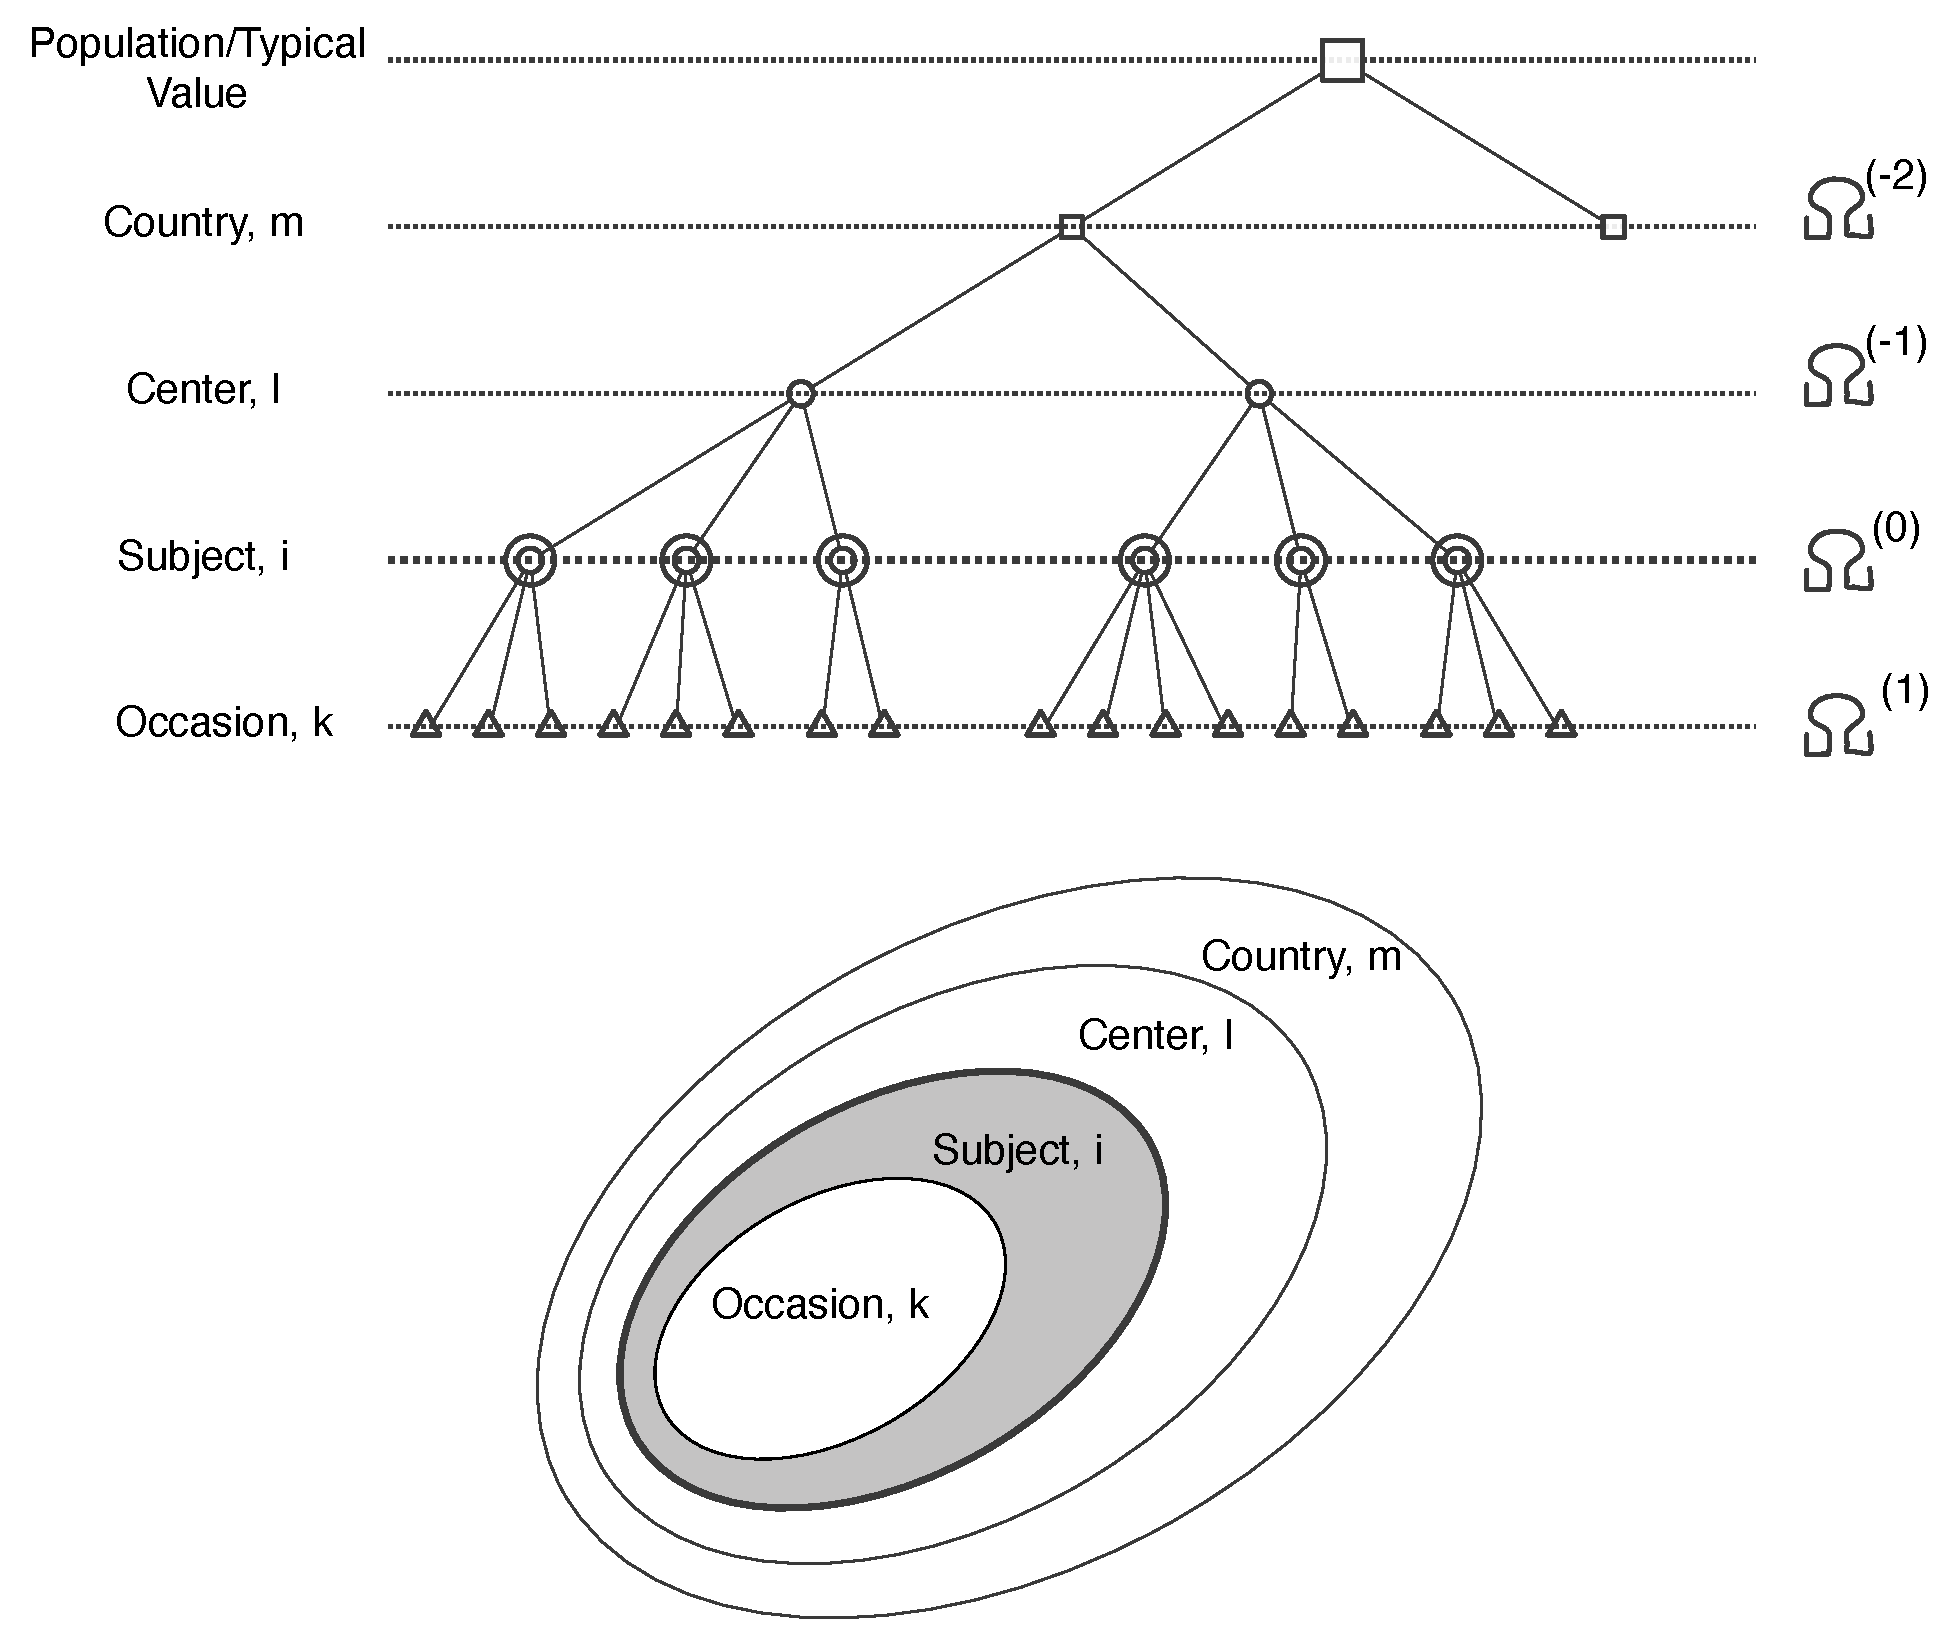
\includegraphics[width=120mm]{pics/tree_IOV2}
 \caption{Example 2 -- four levels of variability:  \{\textit{country (-2), centre (-1), subject (0), occasion (+1)}\}}
 \label{tree_IOV2}
 \end{figure}

